

Im ersten Schritt soll die Formular-Anwendung  in ihrer Grundstruktur entwickelt werden. Die erste Ansicht, welche der Benutzer sieht, soll die Übersicht der bereits eingetragenen Maßnahmen sein. Abbildung \ref{fig:Schritt1Uebersicht} zeig diese Übersicht. 
% TODO: rausgekürzt, doch wieder rein nehmen?
%Dort ist auch zu sehen, dass die Anwendung ohne Anpassungen zunächst einmal im sogenannten Material Design\footnoteI{Material Design umfasst eine Reihe von Prinzipien zur Auszeichnung von Benutzeroberflächen. Das ist Design-System wurde von Google Inc. entwickelt.  Der Name leitet sich daher ab, dass Objekte mit der Nachahmung physikalischer Eigenschaften - wie etwa dem Werfen eines Schattens - den Eindruck von tatsächlichen Materialien erwecken. \footnote{\cite{MaterialDesignIntroduction}}} gestylt ist.
\begin{figure}[H]
	\centering
    \includegraphics[width=1.0\textwidth]{Inhalt/Hauptteil/Implementierung/Schritt-1/Übersicht.png}
	\caption[Schritt 1 Übersicht]{Der Übersicht-Bildschirm zeigt in  Schritt 1 zunächst nur die Maßnahmen mit ihrem Titel und Bearbeitungsdatum in den Kategorien \enquote{Abgeschlossen} und \enquote{In Bearbeitung}. Quelle: Eigene Abbildung}
	\label{fig:Schritt1Uebersicht}
\end{figure} 
Die Auflistung der Maßnahmen erfolgt in den Kategorien \enquote{In Bearbeitung} und \enquote{Abgeschlossen}. Innerhalb dieser Rubriken werden die Maßnahmen in einer Tabelle angezeigt. Mit einem Klick auf den Button unten rechts im Bild wird der Benutzer auf die zweite Ansicht weitergeleitet: die Eingabemaske. Sie ist in Abbildung \ref{fig:Schritt1Eingabemaske} zu sehen.
\begin{figure}[H]
	\centering
    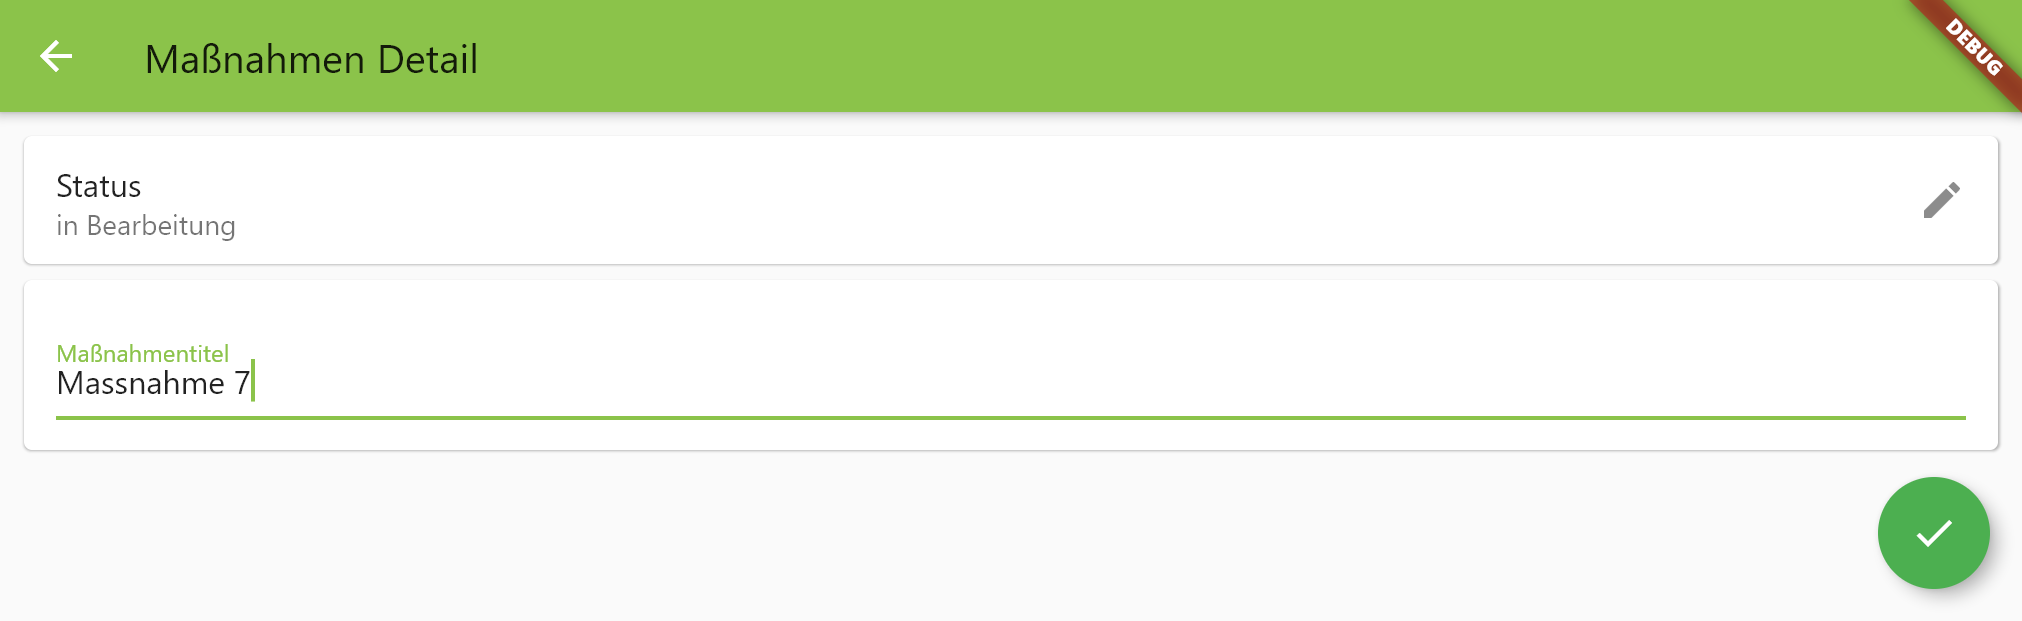
\includegraphics[width=1.0\textwidth]{Inhalt/Hauptteil/Implementierung/Schritt-1/Eingabemaske.png}
	\caption[Schritt 1 Eingabemaske]{Die Eingabemaske zeigt im Schritt 1 eine Karte zum Selektieren des Status und ein Eingabefeld für den Titel. Quelle: Eigene Abbildung}
	\label{fig:Schritt1Eingabemaske}
\end{figure} 
Sie ermöglicht die Eingabe des Maßnahmen-Titels über ein simples Eingabefeld. Darüber hinaus ist die Selektions-Karte für den Status zu sehen. Mit einem Klick auf diese Karte öffnet sich der Selektions-Bildschirm. Er ermöglicht die Auswahl der Auswahloptionen, in diesem Fall die Optionen \enquote{in Bearbeitung} und \enquote{abgeschlossen}, wie in Abbildung \ref{fig:Schritt1SelektionsBildschirmStatus} zu sehen.
\ref{fig:Schritt1Uebersicht}
\begin{figure}[H]
	\centering
    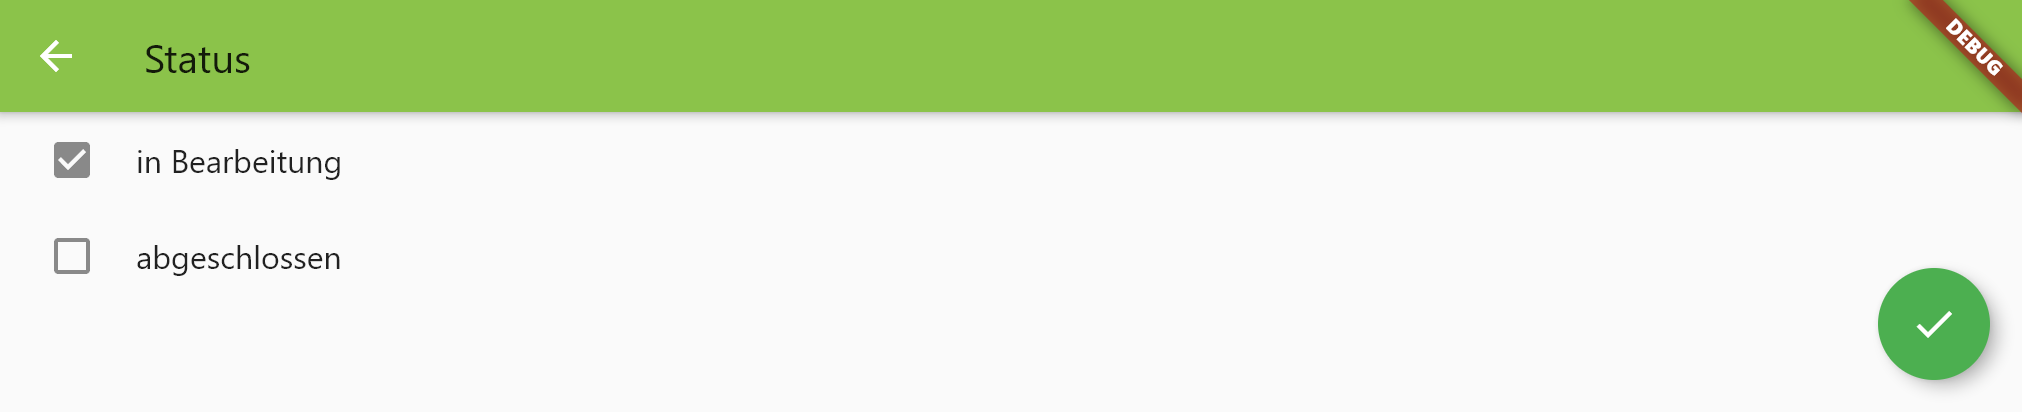
\includegraphics[width=1.0\textwidth]{Inhalt/Hauptteil/Implementierung/Schritt-1/Status Auswahl.png}
	\caption[Schritt 1 Selektions-Bildschirm für Status]{Der Selektions-Bildschirm für das Feld Status erlaubt die Auswahl der Optionen \enquote{in Bearbeitung} und \enquote{abgeschlossen}. Quelle: Eigene Abbildung}
	\label{fig:Schritt1SelektionsBildschirmStatus}
\end{figure}

% TODO: rausgekürzt, doch wieder rein nehmen?
%\footnoteI{Ein floating action button (FAB) ist im Material Design ein Button, der über der Benutzeroberfläche schwebt und daher dem Benutzer leicht ins Auge fällt. Aus diesem Grund wird er für primäre Aktionen genutzt - in diesem Fall dem Erstellen einer neuen Maßnahme. \footnote{\cite{MaterialDesignFloatingActionButton}}} ist in der unteren rechten Ecke der Ansicht zu finden. Mit einem Klick darauf wird der Benutzer auf die zweite Ansicht weitergeleitet: die Eingabemaske. 

\section{HIER EINFÜGEN Status Choice}
\begin{listing}[h]
    \inputminted[firstline=5, lastline=11] {dart}
    {Quellcode/Schritt-1/conditional_form/lib/choices/choices.dart}
\caption[Schritt 1 Klasse LetzterStatus]{Die Klasse LetzterStatus, Quelle: Eigenes Listing, \newline Datei: Quellcode/Schritt-1/conditional_form/lib/choices/choices.dart}
\label{lst:Schritt1KlasseLetzterStatus}
\end{listing} 

\begin{listing}[h]
    \inputminted[firstline=3, lastline=7] {dart}
    {Quellcode/Schritt-1/conditional_form/lib/choices/base/choice.dart}
\caption[Schritt 1 Klasse Choice]{Die Klasse Choice, Quelle: Eigenes Listing, \newline Datei: Quellcode/Schritt-1/conditional_form/lib/choices/base/choice.dart}
\label{lst:Schritt1KlasseChoice}
\end{listing} 

\begin{listing}[h]
  \inputminted[firstline=13] {dart}
  {Quellcode/Schritt-1/conditional_form/lib/choices/choices.dart}
\caption[Schritt 1 Die Menge letzterStatusChoices]{Die Menge letzterStatusChoices, Quelle: Eigenes Listing, \newline Datei: Quellcode/Schritt-1/conditional_form/lib/choices/choices.dart}
\label{lst:Schritt1DieMengeLetzterStatusChoices}
\end{listing} 

\begin{listing}[h]
  \inputminted[firstline=10] {dart}
  {Quellcode/Schritt-1/conditional_form/lib/choices/base/choice.dart}
\caption[Schritt 1 Klasse Choices]{Die Klasse Choices, Quelle: Eigenes Listing, \newline Datei: Quellcode/Schritt-1/conditional_form/lib/choices/base/choice.dart}
\label{lst:Schritt1KlasseChoices}
\end{listing} 

\begin{listing}[h]
\begin{minted}[firstnumber=6]{dart}
part '$file_name$.g.dart';

abstract class $ClassName$ implements Built<$ClassName$, $ClassName$Builder> {
    $todo$
    
    $ClassName$._();
    factory $ClassName$([void Function($ClassName$Builder) updates]) = _$$$ClassName$;
}
\end{minted} 
\caption[built_value Live Template]{Live Template für die Erstellung von built_value Boilerplate-Code in Android Studio, Quelle: Jetbrains Marketplace Built Value Snippets Plugin}
\label{lst:BuiltValueLiveTemplate}
\end{listing}


\section{Ein Test soll verifizieren, dass die Daten korrekt abgelegt werden}



Doch damit die Daten angezeigt und verändert werden können, müssen sie zunächst serialisierbar sein, sodass sie auf einen Datenträger geschrieben und von dort auch wieder gelesen werden können. 
% todo: Serialisierung erklären
Die zwei bekanntesten Bibliotheken zum Serialisieren in Dart heißen json_serializable und built_value.
% todo medium: Vgl. https://flutter.dev/docs/development/data-and-backend/json
% todo medium: Was ist flutter, Flutter nutzt Dart
% todo medium: Model View View Model
Beide haben gemeinsam, dass sie Quellcode generieren, welcher die Umwandlung der Objekte in JSON übernimmt.
% todo: json_serializable erklären
% todo: tree shaking erklären https://flutter.dev/docs/development/data-and-backend/json
built_value bietet im Gegensatz zu JSON Serializable jedoch die Möglichkeit unveränderbare Werte-Typen -  sogenannte immutable value types -  zu erstellen. Da diese  unveränderbaren Werte noch bei der Erstellung des sogenannten ViewModels -  Mehr dazu im Kapitel XXX - hilfreich werden, wurde sich für diese Bibliothek entschieden.
% todo high: Kapitel Referenz einfügen

Ein Werte-Typ für built_value erfordert etwas Boilerplate-Code,  um den generierten Quellcode mit der selbstgeschriebenen Klasse zu verknüpfen.  Dieser Boilerplate-Code kann durch das Live Template für Android Studio in Listing \ref{lst:BuiltValueLiveTemplate} generiert werden. \footnoteL{https://web.archive.org/web/20210710140113/https://github.com/GiancarloCode/built-value-snippets/blob/master/intellij/src/main/resources/liveTemplates/snippets.xml}
% todo medium: live template erklären






\$ClassName\$ Wird dabei jeweils durch den gewünschten Klassennamen ersetzt. Android Studio erlaubt, dass bei Einfügen des live Templates der Klassenname einmalig eingegeben werden muss.  Anschließend wird mithilfe des Templates der Boilerplate Code generiert. In Listing \ref{lst:Schritt1WerteTypMassnahme} ist der Werte-Typ \enquote{Maßnahme} zu sehen. Die Zeilen 11 bis 13, sowie 23 bis 28 wurden dabei automatisch erstellt. Die Zeilen 14 bis 21 wurden hinzugefügt. Zunächst soll die Maßnahme über die \enquote{guid} - Kurzform von General Unique Identifier - eindeutig identifiziert werden können.
%  todo - guid General unique identifier erklären
Die Attribute \enquote{letzteBearbeitung} und \enquote{identifikatoren} sind im Gegensatz zu dem String-Attribut guid zusammengesetzte Datentypen, die im Folgenden weiter beleuchtet werden.

Auffällig ist, dass es sich hier um eine abstrakte Klasse handelt und die drei Attribute jeweils Getter-Methoden ohne Implementierung sind. Eine solche Getter-Methode speichert keinen wert, sondern gibt lediglich den Wert eines Feldes zurück. Die dazugehörigen Felder,  Setter-Methoden, die konkrete Klasse und der restliche generierte Code ist in der gleichnamigen Datei mit der Endung \enquote{.g.dart} (Zeile 11) zu finden.

Die Klassen-Methode \enquote{_initializeBuilder} kann in jedem Werte-Typ hinterlegt werden, um Standardwerte für Felder festzulegen.
% todo medium: Vgl. https://pub.dev/packages/built_value/changelog
Die Methode wird intern von built_value aufgerufen. Bei dem Feld \enquote{guid} handelt es sich um einen String, der keine Null-Werte zulässt. Könnte das Feld auch Null-Werte annehmen, so wäre die Notation in Dart dafür stattdessen \enquote{String? get guid;}. built_value erwartet also immer einen Wert für dieses Feld. Sollte die Datei gelesen werden, welche die Maßnahmen enthält, so enthält jede Maßnahme bei der Deserialisierung den abgespeicherten Wert für die \enquote{guid} und somit wird das Feld gefüllt. Doch sollte eine leere Maßnahme über einen Konstruktor erstellt werden, so wäre das Feld \enquote{guid} leer und built_value würde einen Fehler auslösen. Aus diesem Grund wird in der Zeile 21 für das Feld \enquote{guid} ein Standardwert festgelegt, nämlich eine zufällige  generierte ID die dem Standard Uuid der Version 4 entspricht. 
% todo high:  https://www.ietf.org/rfc/rfc4122.txt
Die Attribute \enquote{letzteBearbeitung} und \enquote{identifikatoren} erhalten dagegen ganz automatisch Standardwerte in Form von Instanzen der dazugehörigen Klassen. Diese wiederum konfigurieren ihre eigenen Felder und deren initialwerte.

\begin{listing}[h]
    \inputminted[firstline=6, lastline=23] {dart}
    {Quellcode/Schritt-1/conditional_form/lib/data_model/massnahme.dart}
\caption[Schritt 1 Werte-Typ Massnahme]{Der Werte-Typ Massnahme, Quelle: Eigenes Listing, \newline Datei: Quellcode/Schritt-1/conditional_form/lib/data_model/massnahme.dart}
\label{lst:Schritt1WerteTypMassnahme}
\end{listing} 

Der Werte-Typ Identifikatoren ist in Listing \ref{lst:Schritt1WerteTypIdentifikatoren} zu sehen.  Er enthält das Attribut \enquote{massnahmenTitel}, welcher im Eingabeformular durch das Texteingabefeld gefüllt werden wird. 

\begin{listing}[h]
    \inputminted[firstline=25, lastline=30] {dart}
    {Quellcode/Schritt-1/conditional_form/lib/data_model/massnahme.dart}
\caption[Schritt 1 Werte-Typ Identifikatoren]{Der Werte-Typ Identifikatoren, Quelle: Eigenes Listing, \newline Datei: Quellcode/Schritt-1/conditional_form/lib/data_model/massnahme.dart}
\label{lst:Schritt1WerteTypIdentifikatoren}
\end{listing} 

Schließlich enthält der Werte-Typ \enquote{LetzteBearbeitung} in Listing \ref{lst:Schritt1WerteTypLetzteBearbeitung} noch die Attribute \enquote{letztesBearbeitungsDatum} in Zeile 43 und \enquote{letzterStatus} in Zeile 50. Im Eingabeformular wird der Selektions-Bildschirm den Inhalt des Feldes \enquote{letzterStatus} Bestimmen. Der initiale Wert auf wird in Zeile 54 auf einen konstanten Wert gesetzt, der dem Zustand \enquote{in Bearbeitung} entspricht - mehr dazu im Kapitel CCCCCCCC.
% todo high: Kapitel Choices einfügen

Das Attribut \enquote{letztesBearbeitungsDatum} ist dagegen nicht im Formular änderbar, sondern wird einmalig in Zeile 53 auf den aktuellen Zeitstempel gesetzt. Zugehörig zu diesem Attribut gibt es noch eine abgeleitete Eigenschaft namens \enquote{formattedDate} (Zeilen 45-48).  Es ist eine Hilfsmethode, die das letzte Bearbeitungsdatum in ein für Menschen lesbares Datumsformat umwandelt. In dem Übersichts-Bildschirm Abbildung \ref{fig:Schritt1Uebersicht} ist das Datumsformat sichtbar.

Da diese Getter-Methode eine Implementierung besitzt, wird für sie von built_value kein Quellcode für die Serialisierung generiert.



\begin{listing}[h]
    \inputminted[firstline=41, lastline=54] {dart}
    {Quellcode/Schritt-1/conditional_form/lib/data_model/massnahme.dart}
\caption[Schritt 1 Werte-Typ LetzteBearbeitung]{Der Werte-Typ LetzteBearbeitung, Quelle: Eigenes Listing, \newline Datei: Quellcode/Schritt-1/conditional_form/lib/data_model/massnahme.dart}
\label{lst:Schritt1WerteTypLetzteBearbeitung}
\end{listing}


\begin{listing}[h]
    \inputminted[firstline=10, lastline=12] {dart}
    {Quellcode/Schritt-1/conditional_form/lib/data_model/serializers.dart}
\caption[Schritt 1 Serializers]{Der Serialisierer für Massnahme und Storage, Quelle: Eigenes Listing, \newline Datei: Quellcode/Schritt-1/conditional_form/lib/data_model/serializers.dart}
\label{lst:Schritt1Serialisierer}
\end{listing} 

 

% Storage Klasse zeigen und beschreiben
% serializers Klasse zeigen und beschreiben
% Korrigieren (Unten)
Wird nun der Befehl \texttt{flutter pub run build_runner build} ausgeführt, so wird der Quellcode generiert und die Werte-Typen können für die Serialisierung genutzt werden. 

Das Ergebnis der Serialisierung wird im dazugehörigen Unit-Test ersichtlich. Listing ZZZZZZZ zeig den Unit Test für den Typ Maßnahme.
In Zeile 8 wird ein Objekt der Klasse Massnahme instanzieiert. Anders als bei gewöhnlichen Datentypen lassen sich bei diesem unveränderlichen Datentyp keine Attribute nach der Erstellung anpassen. Die einzige Möglichkeit besteht darin, ein neues Objekt  mit dem gewünschten Attributwert zu erstellen und die  restlichen Werte des alten Objektes zu übernehmen.  dies ist in Bild Vaio mithilfe des sogenannten Bilder Entwurfsmuster möglich. In den Zeilen 9 bis 10 wird so ein neues Objekt von der Klasse Maßnahme mit Hilfe der Methode rebuild erzeugt und anschließend der Referenz Maßnahme zugewiesen, wodurch sie ihren alten Wert verliert.

 



\begin{listing}[h]
    \inputminted[firstline=6, lastline=23] {dart}
    {Quellcode/Schritt-1/conditional_form/test/data_model/massnahme_test.dart}

\caption[Schritt 1 Maßnahme serialisiert ohne Fehler Unit-Test]{Ein automatisierter Testfall überprüft, ob die Maßnahme korrekt serialisiert wird, Quelle: Eigenes Listing, \newline Datei: Quellcode/Schritt-1/conditional_form/test/data_model/massnahme_test.dart}

\label{lst:MaßnahmeSerialisiertOhneFehlerUnitTest}

\end{listing}

\begin{listing}[h]
    \inputminted[firstline=36, lastline=56] {dart}
    {Quellcode/Schritt-1/conditional_form/test/data_model/massnahme_test.dart}

\caption[Schritt 1 Maßnahme deserialisiert ohne Fehler Unit-Test]{Ein automatisierter Testfall überprüft, ob die Maßnahme korrekt deserialisiert wird, Quelle: Eigenes Listing, \newline Datei: Quellcode/Schritt-1/conditional_form/test/data_model/massnahme_test.dart}

\label{lst:MaßnahmeDeserialisiertOhneFehlerUnitTest}

\end{listing}

 



\begin{listing}[h]
    \inputminted[firstline=9, lastline=21] {dart}
    {Quellcode/Schritt-1/conditional_form/lib/data_model/storage.dart}

\caption[Schritt 1 Werte-Typ Storage]{Der Werte-Typ Storage, Quelle: Eigenes Listing, \newline Datei: Quellcode/Schritt-1/conditional_form/lib/data_model/storage.dart}

\label{lst:Schritt1WerteTypStorage}

\end{listing}




\begin{listing}[h]
    \inputminted[firstline=7, lastline=31] {dart}
    {Quellcode/Schritt-1/conditional_form/test/data_model/storage_test.dart}

\caption[Schritt 1 Maßnahmen deserialisieren ohne Fehler Unit-Test]{Ein automatisierter Testfall überprüft, ob die Liste der Maßnahmen korrekt serialisiert wird, Quelle: Eigenes Listing, 
\newline Datei: Quellcode/Schritt-1/conditional_form/test/data_model/storage_test.dart}

\label{lst:Schritt1MaßnahmenSerialisierenOhneFehlerUnitTest}

\end{listing}



\begin{listing}[h]
    \inputminted[firstline=48, lastline=75] {dart}
    {Quellcode/Schritt-1/conditional_form/test/data_model/storage_test.dart}

\caption[Schritt 1 Maßnahmen deserialisieren ohne Fehler Unit-Test]{Ein automatisierter Testfall überprüft, ob die Liste der Maßnahmen korrekt deserialisiert wird, Quelle: Eigenes Listing, 
\newline Datei: Quellcode/Schritt-1/conditional_form/test/data_model/storage_test.dart}

\label{lst:Schritt1MaßnahmenDeserialisierenOhneFehlerUnitTest} 

\end{listing}





\begin{listing}[h]
    \inputminted[firstline=7, lastline=31] {dart}
    {Quellcode/Schritt-1/conditional_form/lib/persistence/massnahmen_json_file.dart}

\caption[Schritt 1 Klasse MassnahmenJsonFile]{Die Klasse MassnahmenJsonFile, Quelle: Eigenes Listing, \newline Datei: Quellcode/Schritt-1/conditional_form/lib/persistence/massnahmen_json_file.dart}

\label{lst:Schritt1KlasseMassnahmenJsonFile}

\end{listing} 

\begin{listing}[h]
\inputminted[firstline=7] {dart}
{Quellcode/Schritt-1/conditional_form/lib/data_access/massnahmen_pool.dart}

\caption[Schritt 1 Klasse MassnahmenPool]{Die Klasse MassnahmenPool, Quelle: Eigenes Listing, \newline Datei: Quellcode/Schritt-1/conditional_form/lib/data_access/massnahmen_pool.dart}

\label{lst:Schritt1KlasseMassnahmenPool}

\end{listing} 















\begin{listing}[htbp]
    \begin{minted}[firstnumber=13]{dart}
final createNewMassnahmeButtonKey = GlobalKey();

class MassnahmenMasterScreen extends StatelessWidget {
  static const routeName = '/massnahmen_master';

  const MassnahmenMasterScreen({Key? key}) : super(key: key);

  @override
  Widget build(BuildContext context) {
    final massnahmenPool = Provider.of<MassnahmenPool>(context, listen: false);

    return Scaffold(
      appBar: AppBar(
        title: const Text('Maßnahmen Master'),
      ),
      body: StreamBuilder<Storage>(
          stream: massnahmenPool.storageSubject,
          builder: (context, _) {
            return SingleChildScrollView(...);
          }),
      floatingActionButton: FloatingActionButton(
          key: createNewMassnahmeButtonKey,
          child: const Icon(
            Icons.post_add_outlined,
            color: Colors.white,
          ),
          onPressed: () {
            final vm =
                Provider.of<MassnahmenFormViewModel>(context, listen: false);

            vm.model = Massnahme();
            Navigator.of(context).pushNamed(MassnahmenDetailScreen.routeName);
          }),
    );
  }
}

\end{minted}
\caption[Schritt 1 Klasse MassnahmenMasterScreen Struktur]{Die Struktur der Klasse MassnahmenMasterScreen, Quelle: Eigenes Listing, \newline Datei: Quellcode/Schritt-1/conditional_form/lib/screens/massnahmen_master.dart}

\label{lst:Schritt1KlasseMassnahmenMasterScreenStruktur}
\end{listing}



    \begin{listing}[htbp]
        \begin{minted}[firstnumber=31]{dart}
return SingleChildScrollView(
  child: Column(
    crossAxisAlignment: CrossAxisAlignment.start,
    children: [
      const Padding(
        padding: EdgeInsets.all(16.0),
        child: Text(
          "Abgeschlossen",
          style: TextStyle(fontSize: 20),
        ),
      ),
      SingleChildScrollView(
          scrollDirection: Axis.horizontal,
          child: Padding(
            padding: const EdgeInsets.all(16.0),
            child: MassnahmenTable(
                massnahmenPool.storage.massnahmen
                    .where((m) =>
                        m.letzteBearbeitung.letzterStatus ==
                        LetzterStatus.fertig.abbreviation)
                    .toSet(), onSelect: (selectedMassnahme) {
              final vm = Provider.of<MassnahmenFormViewModel>(
                  context,
                  listen: false);
              vm.model = selectedMassnahme.rebuild((m) => m
                ..letzteBearbeitung.letztesBearbeitungsDatum =
                    DateTime.now().toUtc());
              Navigator.of(context)
                  .pushNamed(MassnahmenDetailScreen.routeName);
            }),
          )),
        \end{minted}
\caption[Schritt 1 Ausgabe der finalen Maßnahmen]{Die Ausgabe der finalen Maßnahmen, Quelle: Eigenes Listing, \newline Datei: Quellcode/Schritt-1/conditional_form/lib/screens/massnahmen_master.dart}

\label{lst:Schritt1AusgabeDerFinalenMaßnahmen}
\end{listing}


\begin{listing}[htbp]
    \begin{minted}[firstnumber=48]{dart}
.where((m) =>
    m.letzteBearbeitung.letzterStatus == LetzterStatus.bearb.abbreviation)
\end{minted}
\caption[Schritt 1 Bedingung der Entwurf-Maßnahmen]{Die Bedingung der Entwurf-Maßnahmen, Quelle: Eigenes Listing, \newline Datei: Quellcode/Schritt-1/conditional_form/lib/screens/massnahmen_master.dart}
\label{lst:Schritt1BedingungDerEntwurfMaßnahmen}
\end{listing}

\begin{listing}[h]
\inputminted[firstline=4] {dart}
{Quellcode/Schritt-1/conditional_form/lib/widgets/massnahmen_table.dart}

\caption[Schritt 1 Klasse MassnahmenTable]{Die Klasse MassnahmenTable, Quelle: Eigenes Listing, \newline Datei: Quellcode/Schritt-1/conditional_form/lib/widgets/massnahmen_table.dart}

\label{lst:Schritt1KlasseMassnahmenTable}

\end{listing} 


    


\begin{listing}[h]
\inputminted[firstline=5] {dart}
{Quellcode/Schritt-1/conditional_form/lib/screens/massnahmen_detail/massnahmen_form_view_model.dart}

\caption[Schritt 1 Klasse MassnahmenFormViewModel]{Die Klasse MassnahmenFormViewModel, Quelle: Eigenes Listing, \newline Datei: Quellcode/Schritt-1/conditional_form/lib/ \newline screens/massnahmen_detail/massnahmen_form_view_model.dart} 

\label{lst:Schritt1KlasseMassnahmenFormViewModel}

\end{listing} 







\begin{listing}[htbp]
    \begin{minted}[firstnumber=10]{dart}
      const saveMassnahmeTooltip = "Validiere und speichere Massnahme";

      class MassnahmenDetailScreen extends StatelessWidget {
        static const routeName = '/massnahmen-detail';
      
        const MassnahmenDetailScreen({Key? key}) : super(key: key);
      
        @override
        Widget build(BuildContext context) {
          final vm = Provider.of<MassnahmenFormViewModel>(context, listen: false);
          final massnahmenPool = Provider.of<MassnahmenPool>(context, listen: false);
      
          Future<bool> saveRecordAndGoBackToOverviewScreen() {...}
      
          Widget createMassnahmenTitelTextFormField(MassnahmenFormViewModel vm) {...}
      
          return Scaffold(
              appBar: AppBar(
                title: const Text('Maßnahmen Detail'),
              ),
              body: WillPopScope(
                onWillPop: () => saveRecordAndGoBackToOverviewScreen(),
                child: Stack(
                  children: [
                    SingleChildScrollView(
                      child: Center(
                        child: Center(
                          child: Padding(
                            padding: const EdgeInsets.all(8.0),
                            child: Column(...),
                          ),
                        ),
                      ),
                    ),
                    Align(
                      alignment: Alignment.bottomRight,
                      child: Padding(
                        padding: const EdgeInsets.all(16.0),
                        child: Column(
                          mainAxisSize: MainAxisSize.min,
                          children: [
                            FloatingActionButton(
                              tooltip: saveMassnahmeTooltip,
                              heroTag: 'save_floating_action_button',
                              child: const Icon(Icons.check, color: Colors.white),
                              onPressed: () =>
                                  saveRecordAndGoBackToOverviewScreen(),
                            )
                          ],
                        ),
                      ),
                    )
                  ],
                ),
              ));
        }
      }
\end{minted}
\caption[Schritt 1 Klasse MassnahmenDetailScreen Struktur]{Die Struktur des Bildschirms MassnahmenDetailScreen, Quelle: Eigenes Listing, Datei: Quellcode/Schritt-1/conditional_form/lib/\newline screens/massnahmen_detail/massnahmen_detail.dart}
\label{lst:Schritt1KlasseMassnahmenDetailScreenStruktur}
\end{listing}


\begin{listing}[h]

  \inputminted[firstline=65, lastline=83] {dart}
  {Quellcode/Schritt-1/conditional_form/lib/screens/massnahmen_detail/massnahmen_detail.dart}

  \caption[Schritt 1 Ausgabe der Formularfelder]{Die Ausgabe der Formularfelder, Quelle: Eigenes Listing, \newline Datei: Quellcode/Schritt-1/conditional_form/lib/\newline screens/massnahmen_detail/massnahmen_detail.dart} 

  \label{lst:Schritt1AusgabeDerFormularfelder}

\end{listing} 

\begin{listing}[h]

  \inputminted[firstline=34, lastline=50] {dart}
  {Quellcode/Schritt-1/conditional_form/lib/screens/massnahmen_detail/massnahmen_detail.dart}

  \caption[Schritt 1 Die Funktion createMassnahmenTitelTextFormField]{Die Funktion createMassnahmenTitelTextFormField, Quelle: Eigenes Listing, \newline Datei: Quellcode/Schritt-1/conditional_form/lib/\newline screens/massnahmen_detail/massnahmen_detail.dart} 

  \label{lst:Schritt1DieFunktionCreateMassnahmenTitelTextFormField}

\end{listing} 

\begin{listing}[h]

  \inputminted[firstline=22, lastline=32] {dart}
  {Quellcode/Schritt-1/conditional_form/lib/screens/massnahmen_detail/massnahmen_detail.dart}

  \caption[Schritt 1 Die Funktion saveRecordAndGoBackToOverviewScreen]{Die Funktion saveRecordAndGoBackToOverviewScreen, Quelle: Eigenes Listing, \newline Datei: Quellcode/Schritt-1/conditional_form/lib/\newline screens/massnahmen_detail/massnahmen_detail.dart} 

  \label{lst:Schritt1SaveRecordAndGoBackToOverviewScreen}

\end{listing} 

\begin{listing}[h]
  \inputminted[firstline=3] {dart}
  {Quellcode/Schritt-1/conditional_form/integration_test/driver.dart}

  \caption[Schritt 1 Integration Test Driver]{Der Integration Test Driver, Quelle: Eigenes Listing, \newline Datei: Quellcode/Schritt-1/conditional_form/integration_test/driver.dart} 

  \label{lst:Schritt1IntegrationTestDriver}

\end{listing} 
  

\begin{listing}[h]
  
  \inputminted[firstline=18, lastline=28] {dart}
  {Quellcode/Schritt-1/conditional_form/integration_test/app_test.dart}

  \caption[Schritt 1 Integrations Test Initialisierung]{Initialisierung des Integrations Tests, Quelle: Eigenes Listing, \newline Datei: Quellcode/Schritt-1/conditional_form/integration_test/app_test.dart} 

  \label{lst:Schritt1IntegrationsTestInitialisierung}

\end{listing}


\begin{listing}[h]
  
  \inputminted[firstline=30, lastline=49] {dart}
  {Quellcode/Schritt-1/conditional_form/integration_test/app_test.dart}

  \caption[Schritt 1 Integrations Test Widget Initialisierung]{Initialisierung des Widgets für den Integrations Tests, Quelle: Eigenes Listing, \newline Datei: Quellcode/Schritt-1/conditional_form/integration_test/app_test.dart} 

  \label{lst:Schritt1IntegrationsTestWidgetInitialisierung}

\end{listing}

\begin{listing}[h]
  
  \inputminted[firstline=51, lastline=68] {dart}
  {Quellcode/Schritt-1/conditional_form/integration_test/app_test.dart}

  \caption[Schritt 1 Hilfsmethode tabSelectionCard]{Die Hilfsmethode tabSelectionCard, Quelle: Eigenes Listing, \newline Datei: Quellcode/Schritt-1/conditional_form/integration_test/app_test.dart} 

  \label{lst:Schritt1HilfsmethodeTabSelectionCard}

\end{listing}



\begin{listing}[h]
  
  \inputminted[firstline=76, lastline=97] {dart}
  {Quellcode/Schritt-1/conditional_form/integration_test/app_test.dart}

  \caption[Schritt 1 Hilfsmethode tabOption]{Die Hilfsmethode tabOption, Quelle: Eigenes Listing, \newline Datei: Quellcode/Schritt-1/conditional_form/integration_test/app_test.dart} 

  \label{lst:Schritt1HilfsmethodeTabOption}

\end{listing}



\begin{listing}[h]
  
  \inputminted[firstline=99, lastline=109] {dart}
  {Quellcode/Schritt-1/conditional_form/integration_test/app_test.dart}

  \caption[Schritt 1 Hilfsmethode fillTextFormField]{Die Hilfsmethode fillTextFormField, Quelle: Eigenes Listing, \newline Datei: Quellcode/Schritt-1/conditional_form/integration_test/app_test.dart} 

  \label{lst:Schritt1HilfsmethodeFillTextFormField}

\end{listing}




\begin{listing}[h]
  
  \inputminted[firstline=111, lastline=117] {dart}
  {Quellcode/Schritt-1/conditional_form/integration_test/app_test.dart}

  \caption[Schritt 1 Button zum Kreieren einer Maßnahme wird ausgelöst]{Der Button zum Kreieren einer Maßnahme wird ausgelöst, \newline Quelle: Eigenes Listing, Datei: Quellcode/Schritt-1/conditional_form/integration_test/app_test.dart} 

  \label{lst:Schritt1ButtonKreierenMaßnahmeAusgeloest}

\end{listing}

\begin{listing}[h]
  
  \inputminted[firstline=119, lastline=120] {dart}
  {Quellcode/Schritt-1/conditional_form/integration_test/app_test.dart}

  \caption[Schritt 1 Letzter Status wird ausgewählt]{Der letzte Status wird ausgewählt, Quelle: Eigenes Listing, \newline Datei: Quellcode/Schritt-1/conditional_form/integration_test/app_test.dart} 

  \label{lst:Schritt1LetzterStatusWirdAusgewählt}

\end{listing}


\begin{listing}[h]
  
  \inputminted[firstline=122, lastline=125] {dart}
  {Quellcode/Schritt-1/conditional_form/integration_test/app_test.dart}

  \caption[Schritt 1 Maßnahmentitel wird eingegeben]{Der Maßnahmentitel wird eingegeben, Quelle: Eigenes Listing, \newline Datei: Quellcode/Schritt-1/conditional_form/integration_test/app_test.dart} 

  \label{lst:Schritt1MaßnahmentitelWirdEingegeben}

\end{listing}



\begin{listing}[h]
  
  \inputminted[firstline=127, lastline=129] {dart}
  {Quellcode/Schritt-1/conditional_form/integration_test/app_test.dart}

  \caption[Schritt 1 Button zum Speichern wird ausgelöst]{Der Button zum Speichern wird ausgelöst, Quelle: Eigenes Listing, \newline Datei: Quellcode/Schritt-1/conditional_form/integration_test/app_test.dart} 

  \label{lst:Schritt1ButtonZumSpeichernWirdAusgelöst}

\end{listing}

\begin{listing}[h]
  
  \inputminted[firstline=131, lastline=143] {dart}
  {Quellcode/Schritt-1/conditional_form/integration_test/app_test.dart}

  \caption[Schritt 1 Ergebnis wird verglichen]{Der Button zum Speichern wird ausgelöst, Quelle: Eigenes Listing, \newline Datei: Quellcode/Schritt-1/conditional_form/integration_test/app_test.dart} 

  \label{lst:Schritt1ErgebnisWirdVerglichen}

\end{listing}

